
%======================问题介绍====================================
\section{Introduction}
With the rapid progress in information technology, people have entered into the epoch with overloaded information. From the prospective of the content provider, it is urgent and necessary to provide accurate and specific information to a particular user, mostly corresponding with his or her personal information and browsing records. Such an system is commonly considered as a automatic recommendation based on data mining, machine learning and statistic models\cite{adomavicius2005toward}. The most well-known and powerful applications of such system in industry fields include Amazon's goods recommendation system, Hulu and NetFlix's film recommendation platform, etc. Actually, no matter we have realized or not, we are experiencing this technology every day. 

In this problem, we are generally required to implement such a film recommendation system based on MovieLens[cite] dataset. The MovieLens dataset provides us with 100,000 records of users' rates to over 1,000 films ranging from 1 to 5. In addition, it offers us with users' fundamental personal identities: ages and occupation. Besides, each films are classified into 19 different themes(romantic, drama, comedy...). On the basis of these information, the problem requires us to realize the following three sub-goals.
\begin{itemize}
\item \textbf{Sub-problem 1:} Establish the users' film favor in mathematical models and analyse some particular users' film characteristic. 
\item \textbf{Sub-problem 2:} Establish the films' theme models and combine with models in Sub-problem 1 to recommend 5 films for users mentioned above.  
\item\textbf{ Sub-problem 3:} Realize a recommendation system for new users with only register information.
\end{itemize} 

We solve sub-problem 1 by modelling users' feature and films' feature and analysing the relationship between them. In sub-problem 2 and 3, we furthermore try to determine the analytical numerical model between the combination of users, film feature and the final rating score by SVM and C\&RT. Finally we test and compare our model with state-of-the-art: collaborative filtering algorithm.

The structure of the paper is organized by three sub-problems, respectively. In each sub-problem, we give our own assumptions, models and experiment results. The final conclusion is given in section 5. The codes and are shown in Appendix. 

\section{Solution for sub-problem 1}
\subsection{Analysis and Assumptions}
In this sub-problem, our goal is to analyse the film preference model for a specific user. Due to the fact that this sub-problem's target object are some specified individuals, we assume that this sub-problem is meant to exhibit the basic preference for each user. In other words, our ultimate output of this goal is giving out each user's subjective film favor. Thus, there is no need to calculate and deduce the overall preference of all users. The most fundamental idea is to simply add the user's rate together and calculate the average value to represent his or her preference. 

Nonetheless, when we recall the actual rating situation: one film may score an abnormal average lower score under thousands of rates due to various reasons(actors, directors, backgrounds, etc), although, its theme satisfies one particular user's favor well. In this degree, we assume that if a film's average score is low whereas our target user gives a "High Five" for it, the reason lies on he or her \textit{is fascinated by} the films' theme. Therefore, the model should reflect this idea and gives a heavier weight when this situation occurs. In addition, the summation of user's preference on all film themes should be one, naturally, it means a normalization operation. 

According to analysis above, we summarize our assumptions as below:
\begin{itemize}
\item \textbf{Assumption 1-1:} The user's preference has nothing to do with his or her age, occupation, merely depend on his or her history rating results.

\item \textbf{Assumption 1-2:} The higher the ratio between the user's score to a film and its average score, the deeper the user prefers it.

\item\textbf{Assumption 1-3:} The summation of one individual's preference on all the themes should be 1.
\end{itemize} 

\subsection{Models}
Suppose we have the film set $F=(f_{1},f_{2},\ldots,f_{n})$, which collects all the films mentioned in the dataset and $U=(u_{1},u_{2},\ldots,u_{m})$ to denote user set. For each rating record, it is merely a dual function between $U$ and $F$, we define $R(i,j)$ is user $u_{i}'s$ rate to film $f_{j}$. 

\begin{equation}
R(i,j)=\begin{cases}
0&\text{no rating record in dataset from $u_{i}$ to $m_{j}$},\\
score&
\text{exist rating record in dataset from $u_{i}$ to $m_{j}$}.
\end{cases}
\end{equation}

First, we calculate the general average score $Avg_{f_{j}}$ for each film in film set. 
\begin{equation}
AVG(f_{j})=\sum^{m}_{i=1}\dfrac{R(i,j)}{count(R(i,j)\neq0)}
\end{equation}
Then, we calculate the summation of "scaled-version" rate score multiplied  by a film-style "mask-vector" $S(f_{j})$, a $s-$ length binary vector defined in file:$u.item$(in this case s equals to 18):
\begin{equation}
UFEAT(u_{i})'=\sum^{n}_{j=1}\dfrac{S(f_{j})*R(i,j)}{AVG(f_{j})}
\end{equation}
After normalized the summation of each dimension in $UFEAT(u_{i})'$ to 1, just as mentioned in\textbf{Assumption 1-3}, we seize the answer in this sub-problem: $UFEAT(u_{i})$. 

\subsection{Experiment Result}
The matrix for specialized 10 people(108, 133, 228, 232, 336, 338, 545, 613, 696, 777) can been viewed in table 1: for a particular user, we quantify his or her film favor in a column. For example, user 108 prefers Drama(0.18) at most, and we can deduce that user 108 has never rate and appreciate Fantasy, Film-Noir and Horror films(their indexes are zero). In addition, we visualize the answer for user 108 and user 133 in figure 1.
\begin{table}
\begin{tabular}{rrrrrrrrrrr}

           &        108 &        133 &        228 &        232 &        336 &        338 &        545 &        613 &        696 &        777  \\  \hline

    Action &      0.13  &      0.12  &      0.06  &      0.08  &      0.08  &      0.03  &      0.20  &      0.10  &      0.06  &      0.06  \\

 Adventure &      0.08  &      0.05  &      0.08  &      0.04  &      0.04  &      0.02  &      0.13  &      0.05  &      0.03  &      0.02  \\

 Animation &      0.01  &      0.00  &      0.00  &      0.01  &      0.00  &      0.03  &      0.03  &      0.02  &      0.00  &      0.01  \\

  Children &      0.02  &      0.07  &      0.05  &      0.03  &      0.02  &      0.01  &      0.05  &      0.02  &      0.00  &      0.01  \\

    Comedy &      0.12  &      0.11  &      0.06  &      0.12  &      0.44  &      0.21  &      0.11  &      0.09  &      0.04  &      0.22  \\

     Crime &      0.02  &      0.03  &      0.02  &      0.03  &      0.03  &      0.02  &      0.02  &      0.07  &      0.08  &      0.04  \\

Documentary &      0.00  &      0.00  &      0.00  &      0.01  &      0.00  &      0.00  &      0.00  &      0.00  &      0.00  &      0.00  \\

     Drama &      0.18  &      0.19  &      0.38  &      0.29  &      0.12  &      0.22  &      0.08  &      0.25  &      0.38  &      0.32  \\

   Fantasy &      0.00  &      0.02  &      0.00  &      0.01  &      0.00  &      0.00  &      0.01  &      0.00  &      0.00  &      0.00  \\

 Film-Noir &      0.00  &      0.00  &      0.00  &      0.01  &      0.00  &      0.03  &      0.00  &      0.02  &      0.02  &      0.00  \\

    Horror &      0.00  &      0.01  &      0.03  &      0.00  &      0.01  &      0.01  &      0.04  &      0.01  &      0.04  &      0.02  \\

  Musician &      0.03  &      0.00  &      0.00  &      0.04  &      0.01  &      0.01  &      0.03  &      0.00  &      0.00  &      0.01  \\

   Mystery &      0.02  &      0.05  &      0.01  &      0.02  &      0.01  &      0.06  &      0.01  &      0.02  &      0.10  &      0.01  \\

   Romance &      0.14  &      0.09  &      0.11  &      0.13  &      0.13  &      0.16  &      0.06  &      0.09  &      0.07  &      0.06  \\

    Sci-Fi &      0.08  &      0.08  &      0.02  &      0.06  &      0.03  &      0.03  &      0.09  &      0.08  &      0.00  &      0.03  \\

  Thriller &      0.08  &      0.12  &      0.06  &      0.05  &      0.05  &      0.09  &      0.08  &      0.09  &      0.11  &      0.10  \\

       War &      0.07  &      0.05  &      0.11  &      0.07  &      0.01  &      0.06  &      0.05  &      0.07  &      0.08  &      0.10  \\

   Western &      0.00  &      0.00  &      0.00  &      0.01  &      0.02  &      0.01  &      0.02  &      0.02  &      0.00  &      0.00  \\

\end{tabular}
\caption{The analytical result for specific users' preference}  
\end{table}
\begin{figure}[htbp]
\centering
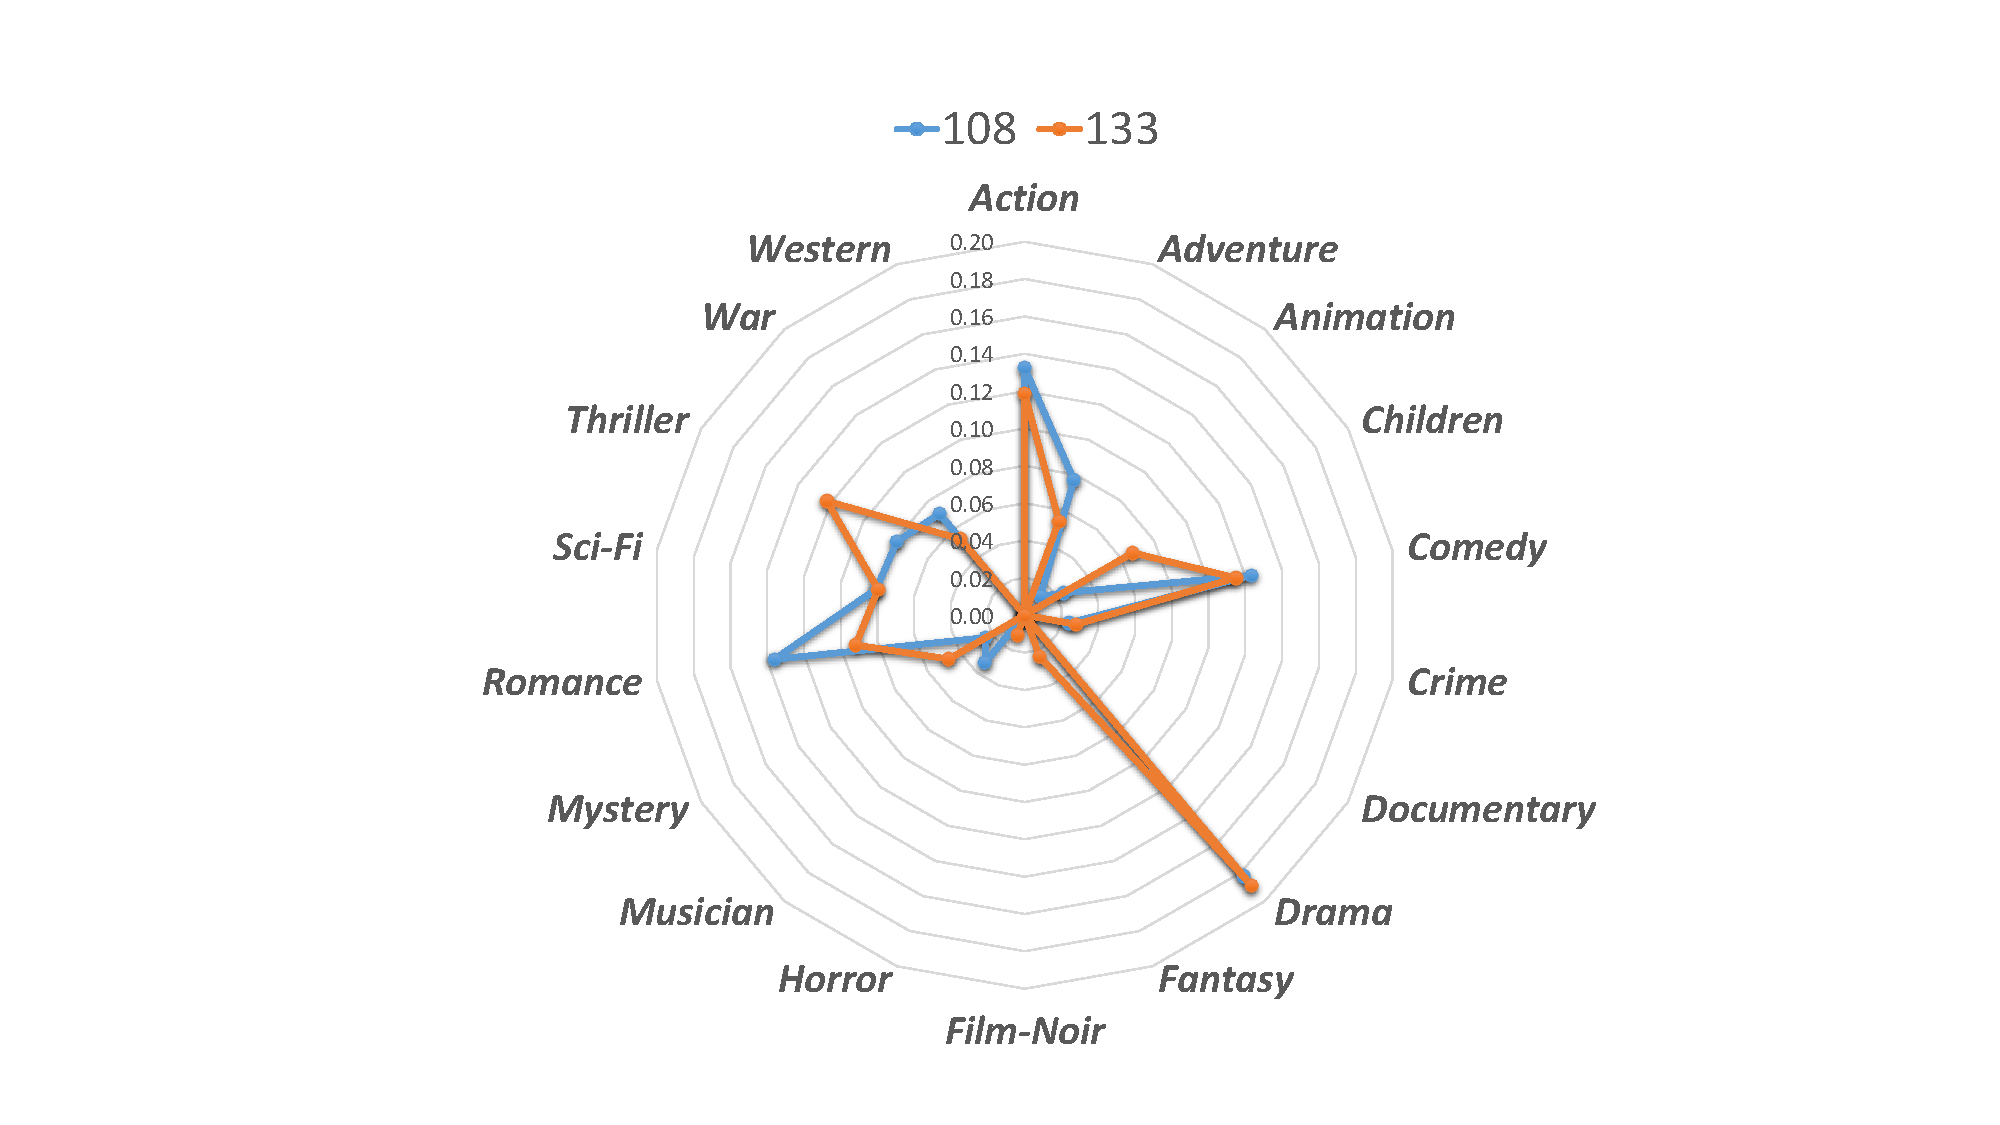
\includegraphics[width=12cm]{/figure/fig1.pdf}
\caption{The rader figure of two user preference} \label{fig:1}
\end{figure}

\section{Solution for sub-problem 2}
\subsection{Analysis and Assumptions}
In sub-problem 2, the demand is even more critical: we need to exploit the internal information for each film and eventually implement the function of recommend five books for specific users. In this aspect, our model is implemented in two steps: the first step is to modelling film datasets; the second is to exploring the relationship between film model and user model with the aid of rating records.

First, let us consider the film-modelling task, which is similar as the one in sub-problem 1. In order to simplify the model, we give such an assumption just like the one mentioned before\cite{jung2012attribute}:

\begin{itemize}
\item \textbf{Assumption 2-1:} Each film can been appreciated from the following angles for a single individual separately: personal preference, age and occupation.
\end{itemize} 


We construct three relationships between film and personal characteristics: film-theme favor, film-age and film-occupation. The first relationship is calculated as a "user-preference weight score".
For a particular film $f_{j}$, we deduce its film-theme favor as follow:
\begin{equation}
FFEAT(f_{j})_{favor}=\dfrac {\sum ^{m}_{i=1}S\left( f_{j}\right) \times R\left( i,j\right) \times UFEAT\left( u_{i}\right) }{\sum ^{m}_{i=1}UFEAT\left( u_{i}\right) }
\end{equation}
In order to seize film-age feature, we manually divide ages into six parts:0~16, 17~24, 25~32, 33~40, 41~48 and over 49, indexed from 1 to 6, respectively. The film-age feature is then calculated by simply counting the average rating scores in each age groups and finally we are able to get the 6-dimension feature: $FFEAT(f_{j})_{age}$. The same idea is applied on acquiring $FFEAT(f_{j})_{occupation}$, a 21-dimension vector(the number of occupation provided in $u.data$ is 21. Finally, we combine $FFEAT(f_{j})_{favor}, FFEAT(f_{j})_{age}, FFEAT(f_{j})_{occupation}$ together as $FFEAT(f_{j})$, which is the model of all films. 

The second task is explore the internal relationship between user feature and film feature, which is the core of the whole system. We give a assumption as following:
\begin{itemize}
\item \textbf{Assumption 2-2:} A pair of rating score $R(u_{i},f_{j})$ is a predictable result corresponding with both user feature: $UUFEAT(u_{i})$ and film feature: $FFEAT(f_{j})$. 
\end{itemize} 

Meanwhile, another perspective of this sub-problem is the state-of-the-art method: collaborative filtering algorithm, a user-angle approach\cite{linden2003amazon,breese1998empirical}. The basic idea is that we can always find the similar class users groups by comparing \textit{"similarity degree"} among user features: $UUFEAT(u{i})$. And we design our recommendation system in another way on the basis on the following assumption:
\begin{itemize}
\item \textbf{Assumption 2-3:} Given two users features $UUFEAT(u_{i}), UUFEAT(u_{j})$, if their similarity in quantity is less than one particular threshold given in advance, we can conclude they have similar film preference and should recommend them with counterparts' high-rating films.
\end{itemize}

\subsection{Models}
We employee two heated Machine Learning model to construct our model. And compare the performance with the traditional Collaborative Filtering Algorithm[cite]. We introduce them one-by-one in each subsection. Note that the first two models are based on \textbf{Assumption 2-2} and \textbf{Assumption 2-3}. The last model is a comparing model transplanted from the state-of-the-art.

\subsubsection{Support Vector Machine regression}
The Support Vector Machine(SVM)[cite] is a classical classifier/regression widely used in machine learning, pattern recognition fields[cite]. The basic idea of SVM is quite similar with the one of Linear Regression. Nevertheless, the extended core idea in SVM is the "maximized-margin" theory: suppose we are trying to find a best separation hyperplane in $\mathbb{R}^{n}$, in SVM theory, the best solution should not only meet up the least error, but also maximize the margin among the hyperplane and all the given points. In other words, the hyperplane is carefully restricted in avoid of over-fitting issues.[cite]
In figure 2, we provide a simple case in $\mathbb{R}^{2}$: in this case the third column is the better case compared with the first two columns. 
\begin{figure}[htbp]
\centering
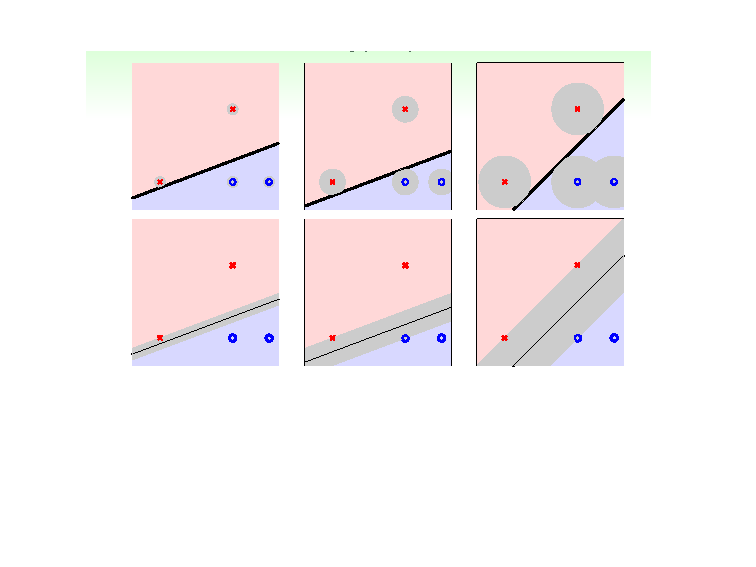
\includegraphics[width=12cm]{/figure/fig2.pdf}
\caption{A simple case of hyperplane choices in $\mathbb{R}^{2}$} \label{fig:2}
\end{figure}

By utilize a batch of records as training data(600000) in $u.data$, we have actually acquired a joint feature of $UUFEAT$ and $FFEAT$, denoted as $\textit{X}={x_{i}|i=1,2,3...p}$ and their regression value $\textit{Y}={y_{i}|i=1,2,3...p}$. We train the SVM parameter $w,b$ by minimize following object function. Actually, the first term is just the common object: least error measure; the second term can be seen as a L2-regularization operation: we want to lower the risk of over-fitting by reduce the norm of $w$. Overall, the objective function is convex and can be solved with convergent solutions.
\begin{equation}
\min _{w,b}\sum ^{p}_{i=1}\left( 1-y_{i}\left( w^{T}x_{i}+b\right) \right) +\dfrac {1}{2}w^{T}w
\end{equation}
In fact, the upper SVM framework has been perfectly implemented by libsvm\cite{chang2011libsvm}, a integral and powerful SVM version in Matlab. We train our SVM model under it with default RBF kernel\cite{chung2003radius} and some other parameter tuning settings. As long as we have acquired $w,b$, for a giving person $u_{i}$, we can calculate all the feature matches $X_{u_{i}}$ by exhausting all the films in dataset and calculating the potential $Y_{u_{i}}$. Eventually, as the problem required, we give out the top-five films with highest predicted rating scores.

\subsubsection{Classification and Regression Tree}
\subsubsection{Collaborative Filtering Algorithm}
As mentioned in \textbf{Assumption 2-3}, the core idea of collaborative filtering algorithm is to calculate the similarity between any given two users with their features. In this case, we synthesize users' preference feature $UUFEAT(u_{i})$, age and occupation together into a ultimate feature vector $UF(u_{i})$. By calculating the Pearson coefficient\cite{hane1993pearson} between $UF(u_{i}), UF(u_{j})$:
\begin{eqnarray}
sim\left(i,j\right) =\dfrac {1}{n-1}\sum ^{n}_{i=1}\left( \dfrac {UF(u_{i})-\overline {UF(u_{i})}}{S_{UF(u_{i})}}\right) \left( \dfrac {UF(u_{j})-\overline {UF(u_{j})}}{S_{UF(u_{j})}}\right) \\
where, \overline {X}=\dfrac {1}{n}\sum ^{n}_{i=1}X_{i} \nonumber \\ 
and, S_{x}=\sqrt {\dfrac {1}{n-1}\sum ^{n}_{i=1}\left( X_{i}-\overline {X}\right) ^{2}} \nonumber 
\end{eqnarray}
we are able to quantify the similarity degree between $u_{i}$ and $u_{j}$.

One particular special step in this model is to calculate the similarity between different jobs, which is normally a non-numerical answer. However, according to the fuzzy theory, we calculate it in semi-quantity form by \textit{Microsoft Bing} search engine: we enter two occupations into search box and take the resultant search items number as their similarity(those items with two mutual occupations). After normalization operation, we achieve Table 2, a symmetric matrix to define occupation similarity.

\begin{longtable}{|r|r|r|r|r|r|r|}
\hline
           & technician &   other &  writer &  executive & administrator &  student \\
\hline
technician &      1.00  &   0.13  &    0.13  &    0.14  &    0.13  &    0.12  \\
\hline
     other &      0.13  &   0.13  &    0.13  &    0.13  &    0.13  &    0.13  \\
\hline
    writer &      0.13  &   0.13  &    1.00  &    0.16  &    0.16  &    0.10  \\
\hline
 executive &      0.14  &   0.13  &    0.16  &    1.00  &    0.10  &    0.16  \\
\hline
administrator &   0.13  &   0.13  &   0.16  &     0.10  &    1.00  &    0.13  \\
\hline
   student &      0.12  &   0.13  &   0.10  &     0.16  &    0.13  &    1.00  \\
\hline
\caption{A part of the occupation similarity matrix.}
\end{longtable}  
Finally, we re-rate all the films in the dataset by the Perason coefficient-weighted sum of all users rates in $u.data$ and sort the top five rating films as result.

\subsection{Experiment Result}
The summary of recommendation result for specific user is shown in Table 3 as below.

\begin{longtable}{|c|c|c|c|}
\hline
{User ID} & {\bf SVM regression(no scaled score)} & {\bf CRT} & {\bf Collaborative filtering(no scaled score)} \\
\hline
\multicolumn{ 1}{|c|}{108} & Film Id: 347 predicted score:4.9245 &            & Film Id: 814 predicted score:5.3837 \\
\hline
\multicolumn{ 1}{|c|}{} & Film Id: 7 predicted score:4.9103 &            & Film Id: 1201 predicted score:5.3081 \\
\hline
\multicolumn{ 1}{|c|}{} & Film Id: 813 predicted score:4.6293 &            & Film Id: 1122 predicted score:4.9761 \\
\hline
\multicolumn{ 1}{|c|}{} & Film Id: 317 predicted score:4.6005 &            & Film Id: 1536 predicted score:4.8043 \\
\hline
\multicolumn{ 1}{|c|}{} & Film Id: 1405 predicted score:4.6005 &            & Film Id: 1293 predicted score:4.5755 \\
\hline
           &            &            &            \\
\hline
\multicolumn{ 1}{|c|}{133} & Film Id: 192 predicted score:4.6002 &            & Film Id: 1122 predicted score:5.0261 \\
\hline
\multicolumn{ 1}{|c|}{} & Film Id: 258 predicted score:4.6002 &            & Film Id: 814 predicted score:5.025 \\
\hline
\multicolumn{ 1}{|c|}{} & Film Id: 193 predicted score:4.6001 &            & Film Id: 1201 predicted score:4.9492 \\
\hline
\multicolumn{ 1}{|c|}{} & Film Id: 64 predicted score:4.6001 &            & Film Id: 1536 predicted score:4.7916 \\
\hline
\multicolumn{ 1}{|c|}{} & Film Id: 357 predicted score:4.6001 &            & Film Id: 1293 predicted score:4.6294 \\
\hline
           &            &            &            \\
\hline
\multicolumn{ 1}{|c|}{228} & Film Id: 1135 predicted score:8.2108 &            & Film Id: 1653 predicted score:4.8226 \\
\hline
\multicolumn{ 1}{|c|}{} & Film Id: 589 predicted score:6.7022 &            & Film Id: 1599 predicted score:4.1469 \\
\hline
\multicolumn{ 1}{|c|}{} & Film Id: 404 predicted score:5.288 &            & Film Id: 1467 predicted score:3.9926 \\
\hline
\multicolumn{ 1}{|c|}{} & Film Id: 14 predicted score:5.1448 &            & Film Id: 1594 predicted score:3.9886 \\
\hline
\multicolumn{ 1}{|c|}{} & Film Id: 742 predicted score:5.0866 &            & Film Id: 1536 predicted score:3.8258 \\
\hline
           &            &            &            \\
\hline
\multicolumn{ 1}{|c|}{232} & Film Id: 56 predicted score:4.6005 &            & Film Id: 1201 predicted score:4.9919 \\
\hline
\multicolumn{ 1}{|c|}{} & Film Id: 1149 predicted score:4.6002 &            & Film Id: 1536 predicted score:4.9518 \\
\hline
\multicolumn{ 1}{|c|}{} & Film Id: 923 predicted score:4.6002 &            & Film Id: 1122 predicted score:4.912 \\
\hline
\multicolumn{ 1}{|c|}{} & Film Id: 48 predicted score:4.6002 &            & Film Id: 814 predicted score:4.8787 \\
\hline
\multicolumn{ 1}{|c|}{} & Film Id: 170 predicted score:4.6002 &            & Film Id: 1599 predicted score:4.7434 \\
\hline
           &            &            &            \\
\hline
\multicolumn{ 1}{|c|}{336} & Film Id: 204 predicted score:4.6004 &            & Film Id: 1467 predicted score:4.0908 \\
\hline
\multicolumn{ 1}{|c|}{} & Film Id: 153 predicted score:4.6003 &            & Film Id: 1599 predicted score:3.8075 \\
\hline
\multicolumn{ 1}{|c|}{} & Film Id: 216 predicted score:4.6002 &            & Film Id: 1189 predicted score:3.7232 \\
\hline
\multicolumn{ 1}{|c|}{} & Film Id: 42 predicted score:4.6002 &            & Film Id: 1536 predicted score:3.4807 \\
\hline
\multicolumn{ 1}{|c|}{} & Film Id: 762 predicted score:4.6002 &            & Film Id: 1594 predicted score:3.3989 \\
\hline
           &            &            &            \\
\hline
\multicolumn{ 1}{|c|}{338} & Film Id: 603 predicted score:4.6005 &            & Film Id: 1536 predicted score:4.8951 \\
\hline
\multicolumn{ 1}{|c|}{} & Film Id: 663 predicted score:4.6005 &            & Film Id: 1201 predicted score:4.8449 \\
\hline
\multicolumn{ 1}{|c|}{} & Film Id: 170 predicted score:4.6003 &            & Film Id: 1599 predicted score:4.8054 \\
\hline
\multicolumn{ 1}{|c|}{} & Film Id: 408 predicted score:4.6003 &            & Film Id: 814 predicted score:4.7241 \\
\hline
\multicolumn{ 1}{|c|}{} & Film Id: 197 predicted score:4.6002 &            & Film Id: 1122 predicted score:4.6906 \\
\hline
           &            &            &            \\
\hline
\multicolumn{ 1}{|c|}{545} & Film Id: 238 predicted score:5.5413 &            & Film Id: 814 predicted score:4.3884 \\
\hline
\multicolumn{ 1}{|c|}{} & Film Id: 121 predicted score:4.6002 &            & Film Id: 1122 predicted score:4.2495 \\
\hline
\multicolumn{ 1}{|c|}{} & Film Id: 257 predicted score:4.6001 &            & Film Id: 1467 predicted score:4.2378 \\
\hline
\multicolumn{ 1}{|c|}{} & Film Id: 472 predicted score:4.6001 &            & Film Id: 1189 predicted score:4.2147 \\
\hline
\multicolumn{ 1}{|c|}{} & Film Id: 230 predicted score:4.6001 &            & Film Id: 1293 predicted score:3.9502 \\

           &            &            &            \\
\hline
\multicolumn{ 1}{|c|}{613} & Film Id: 194 predicted score:4.6004 &            & Film Id: 1536 predicted score:4.918 \\
\hline
\multicolumn{ 1}{|c|}{} & Film Id: 178 predicted score:4.6002 &            & Film Id: 1201 predicted score:4.888 \\
\hline
\multicolumn{ 1}{|c|}{} & Film Id: 887 predicted score:4.6002 &            & Film Id: 1122 predicted score:4.8509 \\
\hline
\multicolumn{ 1}{|c|}{} & Film Id: 750 predicted score:4.6001 &            & Film Id: 814 predicted score:4.8425 \\
\hline
\multicolumn{ 1}{|c|}{} & Film Id: 357 predicted score:4.6001 &            & Film Id: 1293 predicted score:4.6415 \\
\hline
           &            &            &            \\
\hline
\multicolumn{ 1}{|c|}{696} & Film Id: 258 predicted score:4.9815 &            & Film Id: 1201 predicted score:4.9422 \\
\hline
\multicolumn{ 1}{|c|}{} & Film Id: 276 predicted score:4.6344 &            & Film Id: 1536 predicted score:4.8192 \\
\hline
\multicolumn{ 1}{|c|}{} & Film Id: 9 predicted score:4.6002 &            & Film Id: 1122 predicted score:4.8121 \\
\hline
\multicolumn{ 1}{|c|}{} & Film Id: 166 predicted score:4.6001 &            & Film Id: 814 predicted score:4.7529 \\
\hline
\multicolumn{ 1}{|c|}{} & Film Id: 134 predicted score:4.6001 &            & Film Id: 1293 predicted score:4.6233 \\
\hline
           &            &            &            \\
\hline
\multicolumn{ 1}{|c|}{777} & Film Id: 880 predicted score:4.6005 &            & Film Id: 1201 predicted score:4.9848 \\
\hline
\multicolumn{ 1}{|c|}{} & Film Id: 168 predicted score:4.6004 &            & Film Id: 814 predicted score:4.9263 \\
\hline
\multicolumn{ 1}{|c|}{} & Film Id: 56 predicted score:4.5999 &            & Film Id: 1122 predicted score:4.9224 \\
\hline
\multicolumn{ 1}{|c|}{} & Film Id: 87 predicted score:4.5999 &            & Film Id: 1536 predicted score:4.9125 \\
\hline
\multicolumn{ 1}{|c|}{} & Film Id: 117 predicted score:4.5997 &            & Film Id: 1599 predicted score:4.629 \\
\hline
\caption{Recommendation result with RAW score under three models.}
\end{longtable} 

From the table above, we can observe some interesting phenomenon and conclusions. First and foremost, the SVM regression method and Collaborative filtering method give us absolutely different results. In our SVM regression algorithm, we can note that for each person, the recommendation result is quite personalized. When we go on a step further to trace each film by id with $u.item$, we find that they are quite coherence with person's characteristic. To exemplifier this idea, we take User 133 as an instance: user 133 is a 53-year-old engineer; our SVM recommendation system presents film 347(comedy and drama), film 7(drama and sci-fi), film 813(documentary), etc as results. According to our experience, the results are quite coherent with the identity of a middle-age engineer. 

However, when we scan over the results generated by collaborative filtering model, we can find that most users are recommended with similar films(1201,1122,814, etc), although their rank are different. When we further track those films are mostly with very high average rates in their own themes(You can imagine those most heated films like \textit{Titanic, Avater} as examples). Recalling the tip that these data are collected in a relatively short-term time interval(\textbf{September 19th, 1997 through April 22nd, 1998}), this result is also somewhat persuasive. Generally speaking, as far as we are concerned, our own SVM regression model is better than the collaborative model. 

\section{Solution for sub-problem 3}
\subsection{Analysis and Assumptions}
\subsection{Models}
\subsection{Experiment Result}


\section{Conclusion}
In this paper, we successfully implement a automatic film recommendation based on MovieLens dataset. We analysis both users' models and films' models based on the dataset and people's own experience in film-rating experiences. Furthermore, we exploit the deeper relationship between users' models and the films' one; by employing SVM regression model, we beat the collaborative filtering algorithm, the state-of-the-art in default parameter settings. In the further research, we will polish up our system by some other popular and powerful statistical models, such as Convolution Neural Network(CNN)[cite], a powerful weapon in deep learning fields and evaluate their performance with our present framework.

\begin{appendices}
\section{Codes}
\subsection{Codes for sub-problem 1}
\lstinputlisting[language=Matlab]{../code/script_UserAverScore.m}
\subsection{Codes for sub-problem 2, 3}
\lstinputlisting[language=Matlab]{../code/svm_regression_generator.m}
\lstinputlisting[language=Matlab]{../code/svm_regression_generator.m}
\end{appendices}